\documentclass{article}
\usepackage[paperwidth=30cm,paperheight=45cm,bmargin=2cm,lmargin=2cm,rmargin=2cm]{geometry}
\usepackage{array}
\usepackage{url}
\usepackage{tikz}
\usepackage{xcolor}
\usepackage{lmodern}
\usepackage{multicol}
\usepackage{tcolorbox}
\usepackage{ctex}
\usepackage{lipsum}
\usepackage{listings}
\usepackage{subfigure}
\usetikzlibrary{shadows,calc}
\tcbuselibrary{skins,theorems,breakable}

\begin{document}
\title{Java程序设计第一次作业}
\maketitle
模拟醉汉行走,醉汉迈出的每一步的方向和步长都是随机的,每一步可以使用一个矢量来表示,累加可得出醉汉最后走出的距离和方向。通过模拟实验,评估其走路的效率。


\section{Java代码}
\begin{lstlisting}[ language=Java]
      import java.lang.Math;
      import java.io.*;
      import java.nio.file.Paths;
      
      public class HomeWork1 {
          public static void main(String[] args) throws IOException {
              int NUM = 2000;
              double distance = 0, x = 0, y = 0, angle = 0;
              double rou, theta;
              for (int i = 0; i < NUM; i++) {
                  rou = Math.random();
                  theta = 2 * Math.random() * Math.PI;
                  x += rou * Math.cos(theta);
                  y += rou * Math.sin(theta);
                  distance = Math.sqrt(Math.pow(x, 2) + Math.pow(y, 2));
                  angle += theta;
                  System.out.printf("He is at %4.6f    %4.6f\n", x, y);
                  System.out.printf("He has finished %4.6f,theta is %4.6f", distance, angle);
              }
          }
      }
    \end{lstlisting}
\section{结果分析}
\qquad 醉汉走路的模拟图如图1所示,经过500步后,完成了0.06m;经过1000步后,完成了15m;经过1500步之后,完成了22m;经过2000步之后,完成了34m。

经计算,效率分别为:0.12\%,1.5\%,1.47\%,1.7\%。效率实在是低,没事儿还是少喝点酒。
\begin{figure}[!htbp]
\centering
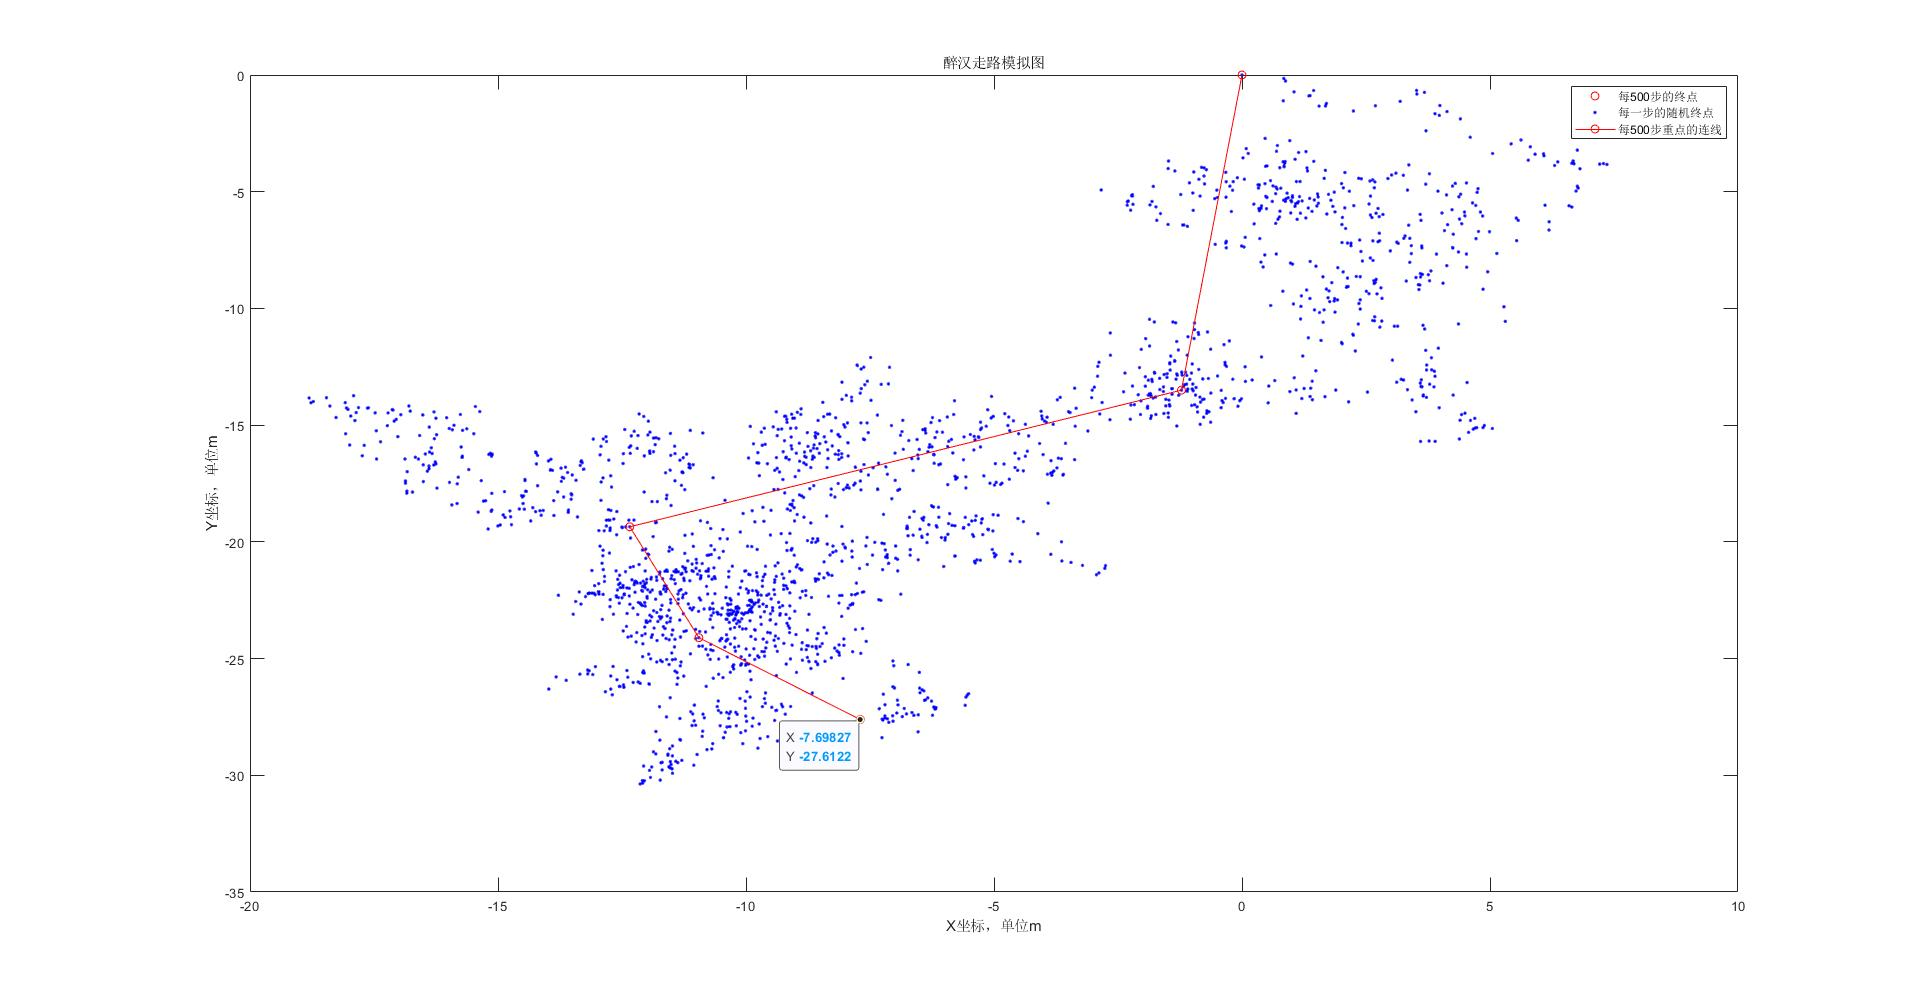
\includegraphics[scale=0.3]{./醉汉.jpg}
\caption{醉汉走路模拟结果,散点为每一步的落点,折线为以500步为间隔的落点,X坐标的范围为[-20,10],Y坐标的范围为[-35,0]}
\end{figure}
\end{document}